\chapter{The argumentative theory of reasoning}
\label{ch:atr}

The argumentative theory of reasoning is Hugo Mercier and Dan Sperber's influential, but not uncontroversial, account of the function of reasoning from an evolutionary perspective. They introduced and coined the theory in a \citeyear{MS11} paper, a culmination of more than a decade's worth of research (\citealp{Sperber01}, \citealp{Sperber10}, \citealp{MS09}).
Briefly, the argumentative theory of reasoning states that the main function of reasoning is to produce arguments and evaluate arguments of others, for the purpose of stabilizing communication.

In this chapter, I will expound the argumentative theory of reasoning by discussing at length each of the precursory papers leading up to \citet{MS11}, in chronological order.
In \cref{sec:Sperber01}, we will discuss Sperber's \citeyear{Sperber01} contribution \emph{An evolutionary perspective on testimony and argumentation}. In \cref{sec:MS09}, we tackle Mercier and Sperber's dual system theory, put forward in the \citeyear{MS09} paper \emph{Intuitive and reflective inferences}.
Next, \cref{sec:Sperber10} sees us discussing \emph{Epistemic vigilance}, a \citeyear{Sperber10} paper by Sperber, Mercier, and colleagues.
By this point, much of the ATR is already laid out.
Finally, in \cref{sec:MS11}, we will summarize the ATR from \citet{MS11}, and briefly discuss the empirical predictions of the theory.

\section{Sperber on the evolution of testimony and argumentation}
\label{sec:Sperber01}

In a \citeyear{Sperber01} paper, Dan Sperber analyzes testimony and argumentation from an evolutionary perspective. In doing so, he provides important groundwork for his later work with Mercier (and others) on the relation between reasoning, argumentation and the stability of communication.

Testimony and argumentation are two concepts central to human communication. Sperber borrows his definitions for these concepts from epistemologist Alvin Goldman, who defines testimony as "the transmission of observed (or allegedly observed) information from one person to others" \citep[p.~401]{Sperber01} and argumentation as "the defense of some conclusion by appeal to a set of premises that provide support for it" (ibid.).
Sperber puts these two concepts in an evolutionary perspective, and discusses in particular how they have figured in stabilizing communication over the course of evolutionary history.

A tempting way to look at communication is as a kind of 'cognition by proxy': through communication, one organism may access information another organism has obtained from its own perception or inference.
For instance, if one vervet monkey expels an alarm call upon observing a leopard in the distance \citep{Seyfarth80}, its conspecifics can through this act of communication benefit from the information derived from the alarmed monkey's perception of the leopard in the distance.
However, Sperber argues that in the case of human communication, testimony does not amount to cognition by proxy. This is because in humans, testimony has different effects than direct perception does. Suppose I observe a leopard in the distance and inform you of this. Upon receiving this testimony, you are in a different cognitive state than you would be if you had perceived the leopard yourself, Sperber argues. Moreover, in human communication, he maintains that interpretation and acceptance of utterances are two separate processes: recognizing what a speaker meant by their utterance is not the same as accepting it as true.\footnote{This may very well be the case philosophically or epistemologically speaking, but psychologically speaking, they may be more intertwined than Sperber implies. In  \citet[\S 3]{Sperber10}, he and his colleagues elaborate more on his stance, making even stronger claims about how comprehension always precedes the acceptance (or rejection) of a claim. Although this is intuitively plausible, see also \citet{Gilbert91} advocating that for someone to comprehend an utterance, they must (at least temporarily) accept it.}

The classical account of animal communication by \citet{DawkinsKrebs78} focuses only on the side of the communicator in the story, maintaining that the function of communication is to manipulate others. Sperber rejects this classical approach, arguing that the interests of the sender cannot be the only driving force in the evolution of communication.
He outlines a similar line of argumentation as we have seen in \cref{sec:S-P08},
arguing that for communication to have stabilized and continued to be stable between senders and receivers, both parties must have benefited from it. In other -- game-theoretic -- terms, communication must (at least in the long run) be a positive-sum game, where both senders and receivers gain from the interaction.

In the case of receiving testimony from others, the receiver gains from testimony "only to the extent that it is a source of genuine (\ldots) information" (p.~404).
On the other side, a sender stands to gain from the production of testimony (and from communication in general) because
\begin{quoting}
    it allows them to have desirable effects on the receivers' attitudes and behavior. By communicating, one can cause others to do what one wants them to do and to take specific attitudes to people, objects, and so on
    \hfill \citep[p.~404]{Sperber01}
\end{quoting}
Sperber later elaborates on this by stating that getting others to accept your communicated message is not intrinsically beneficial. Rather, it is indirectly beneficial, through bringing about these 'desirable effects' in others, as a way of \emph{cognitive manipulation}.
Sperber notes that it is exactly this self-interest of the sender that renders this 'cognition by proxy' view as inapplicable to human communication.
Moreover, he concludes from his observations that
\begin{quoting}
    the function of communication presents itself differently for communicator and audience
    \hfill (p.~411)
\end{quoting}
We return to this conclusion to criticize it in \cref{sec:comm-func-scrutiny}.

Sperber goes on to cast his observations in game-theoretic terms by sketching out a payoff matrix for a one-off communicative event; see \cref{fig:matrix}.

\begin{figure}[ht]
    \centering
    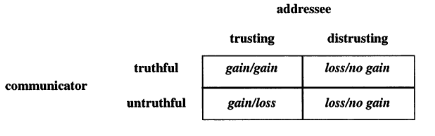
\includegraphics[width=\textwidth]{chapters/img/matrix-sperber.png}
    \caption{Payoff matrix for one-off communicative event}
    \label{fig:matrix}
\end{figure}

In sketching out this scenario, he considers that senders may be truthful or untruthful, and receivers may be trusting or distrusting. According to Sperber, the sender's gain amounts to whether they have the 'desired' effect on the receiver; therefore, the sender gains from the interaction if the receiver is trusting (since this means the sender's message is accepted), and loses from the interaction if the receiver is distrusting. The payoff of this event for the sender is thus independent of the truthfulness of the sender. On the side of the receiver, their payoff \emph{is} dependent on the truthfulness of the sender: the receiver gains if they accept a truthful message, loses if they accept an untruthful message, and incurs no gain nor loss if they are distrusting and thus don't accept a message (truthful or not).

Sperber notes that the optimal strategy for a game like this varies with the circumstances for both players: it is not beneficial to be always truthful, nor always untruthful; nor is it beneficial to be always trusting, nor always distrusting. In other words, there is no one stable solution to this game.
This is especially the case once we move away from this simple one-off communicative event to an iterated game of communication, where not only short-term payoffs but also long-term payoffs determine the optimal strategy.
Therefore, it is in the receiver's interest to calibrate their trust towards senders as accurately as possible; in fact, Sperber argues, this trust calibration is necessary to account for the stability of communication.

Unlike non-human animals, humans can not only communicate facts through testimony; they also have \emph{argumentation} at their disposal. Senders may provide receivers with reasons to accept their testimony; the receiver may then evaluate these reasons and accept or reject the testimony, independent of their trust in the sender.
Sperber notes that reasoning may be used individually for reflection, or socially for communication in dialogical argumentation. He argues that, although classically the former has been viewed as the function of reasoning (cf. \citet{Novaes20}), this is implausible from an evolutionary point of view. He maintains that domain-general reasoning abilities are cognitively costly and slow, and therefore could not have evolved for the purpose of producing knowledge, since more specific mechanisms would better suit this function. Instead, the function of reasoning is communicative rather than individual:
\begin{quoting}
    {[Reasoning]} is an evaluation and persuasion mechanism, not, or at least not directly, a knowledge-production mechanism.
    \hfill \citep[p.~409]{Sperber01}
\end{quoting}

Next, Sperber sketches out the steps in what he calls the 'evaluation-persuasion arms race', i.e., the chain of evolutionary adaptations that has resulted in our mechanisms for argument production and evaluation.
He argues that the first step in this 'arms race' was for the receiver to develop \emph{coherence checking}. Coherence checking involves attending to both the internal coherence of the communicated message, and the external coherence with what the receiver already believes. Coherence checking, Sperber argues, is a useful defense against the risks of being deceived by the sender, because lies and other false claims are often externally or internally incoherent.
The second step in the arms race was then for the sender to anticipate this coherence-checking by overtly displaying the coherence of their message to their receiver, which requires argumentative form; thus, testimony becomes argument.
The next steps in the arms race were then on the side of the receiver to develop skills for examining these displays of coherence (i.e., arguments), and on the side of the sender to 'improve their argumentative skills'.
Mercier and Sperber nicely capture these next steps in the arms race in their \citeyear{MS11} paper, stating that
\begin{quoting}
    receivers' coherence checking creates selective pressure for communicators' coherence displays in the form of arguments, which in turn creates selective pressure for adequate evaluation of arguments on the part of receivers
    \hfill (p.~96)
\end{quoting}

% \todo[inline]{(Add small summary, concluding remark or segue)}

\section{Mercier \& Sperber on intuitive vs. reflective inference}
\label{sec:MS09}

Let us move on to the next stop along the path to the argumentative theory of reasoning. In the \citeyear{MS09} paper \emph{Intuitive and reflective inferences}, Mercier and Sperber propose their own dual system theory of reasoning, in a similar vein to existing dual process theories of reasoning \citep{Sloman96, Evans03, Evans13, Kahneman11}.
They introduce their distinction between intuitive and reflective inferences as part of a massive-modularist framework, which maintains that the mind consists of a number of cognitive modules specialized to specific domains.
This view is certainly not an uncontroversial one (cf. \citet[\S 3.1]{Novaes18}); I consider a detailed discussion of the massively-modularist view of the mind out of scope of this thesis.

Before we consider the contributions by \citet{MS09} however, let me make a slightly anachronistic\todo{Change this word} pivot. In order to clarify some terminology that is not adequately discussed in \citet{MS09}, we briefly turn to a discussion of intuitive inference and argument in \citet[\S 1.1]{MS11}.
There, Mercier and Sperber posit that the processes that are executed by inferential modules are unconscious: though one might be aware of the output of such a process -- its conclusion -- one is unaware of the process itself. In other words, "All inferences carried out by inferential mechanisms are in this sense \emph{intuitive}" \citep[p.~58]{MS11}.
Importantly, they then highlight a distinction between inferences and arguments.
Inferences are processes: they take as input a representation, and they output a representation.
Arguments on the other hand are representations themselves, resulting from inference. They are "the output of an intuitive inferential mechanism"; in particular, they are "representations of relationships between premises and conclusions" \citep[p.~58]{MS11}.
Both inferences and arguments have conclusions, but there is an ontological dissimilarity between these conclusions.
The conclusion of an inference is its output. Characteristically, the output of an inference is justified by the input of the inference; thus, we call this output a conclusion.
The conclusion of an argument, on the other hand, is part of the representation itself, i.e. it is part of the argument.

Pivoting back to Mercier and Sperber's \citeyear{MS09} discussion of intuitive and reflective inferences,
the authors argue that one of the many modules of the mind is the argumentation module, which "provides us with reasons to accept conclusions" (p.~155). The module takes as input a claim, and potentially other information relevant for evaluating this claim, and it produces as its output reasons for accepting or rejecting the claim.
The authors note that the direct output of any inferential module is \emph{intuitive}, in the sense that we accept the module's output without consciously attending to the reasons for this acceptance. This is then also the case for the argumentation module, as it is an inferential module like any other. The direct ('intuitive') output of the argumentation module is then "the representation of an argument-conclusion relationship" (ibid.).
The difference then between intuitively accepting a claim and accepting it because of explicit reasons, is that in the latter case one engages in "disembedding a conclusion from the argument that justifies it" (ibid.).
This disembedded conclusion from the direct output then constitutes the indirect output of the argumentation module.

From this view on the modularity of the mind, and the argumentation module in particular, Mercier and Sperber then develop a dualistic approach to inference.
Their account distinguishes between intuitive inferences on the one hand, and reflective inferences on the other. Reflective inferences are then what Mercier and Sperber refer to as reasoning, or 'reasoning proper'.

Mercier and Sperber emphasize that their dual systems approach is different from the classical distinction between the fast and frugal thinking of system~1 and the slow and analytical thinking of system~2 (cf. \citet{Kahneman11}). They maintain that system~1 and system~2 operate at the same level\footnote{It is unclear what they mean by this comment though; see \citet[p.~156]{MS09}.}, whereas intuitive and reflective inference do not: intuitive inferences are carried out by any module, but reflective inferences result specifically from the argumentation module -- more precisely, reflective inferences are an indirect output of the argumentation module \citep[p.~156]{MS09}.

Moving beyond their dual system approach, Mercier and Sperber go on to provide yet more foundation to their up-and-coming argumentative theory of reasoning by discussing the function of reflective inference -- in other words, the function of reasoning.
Before doing so, they remark that the function of intuitive inference is less controversial than the function of reflective inference (but they do not explicate what this function is).
With regards to the function of reflective inference, they first discuss three 'classical' views on the function of system~2 reasoning.
The first view maintains that system~2 represses system~1's impulses seeking immediate gratification, in order to obtain delayed gratification \citep{Sloman96}. Mercier and Sperber argue that this cannot be the function of reasoning, since non-human animals also possess the ability to delay gratification, but not the ability to reason\footnote{This latter claim is left implicit by Mercier and Sperber in this paper. In \citet[p.~57]{MS11}, they explicate their conviction that non-human animals cannot reason; cf. \citet{Hume39}.}.
Moreover, they argue that empirical case studies discussed in \citet{Damasio94} suggest that abilities for delayed gratification are dissociated from abilities for reasoning.
The second view on the function of reasoning maintains that system~2 reasoning enables us to better deal with novelty \citep{EvansOver1996}.
Mercier and Sperber argue that it is implausible that this is the function of reasoning, since there are other features of human cognition that better explain and support this ability. Moreover, they state that reasoning cannot be said to play a central role in memory and imagination.

These two views on the function of reasoning have in common that they posit that system~2 'compensates' for the shortcomings of system~1.
This idea culminates in the third view on the function of reasoning that Mercier and Sperber discuss. This is the view that the function of reasoning is to enhance individual cognition, or in a stronger version, this view concerns the Cartesian conception of reasoning as '\emph{the} road to knowledge'.
They argue that this is evolutionarily implausible due to a cost-benefit issue.
Reasoning is cognitively costly, and intuitive inference is not so unreliable that using reflective inference instead would be, on the whole, advantageous.

In the remainder of the paper, the authors discuss predictions stemming from their ascribed function of reasoning, and empirical evidence corroborating these predictions. We will return to these and more empirical predictions of the ATR in \cref{sec:MS11}, since Mercier and Sperber's \citeyear{MS11} paper goes into much more detail on this.

\section{Sperber and colleagues on epistemic vigilance}
\label{sec:Sperber10}

% my prologue
Next up is the concept of \emph{epistemic vigilance}, which was introduced by Sperber, Mercier and colleagues in a seminal \citeyear{Sperber10} paper.
This concept constitutes a cornerstone of the argumentative theory of reasoning. We will return to the concept of epistemic vigilance to evaluate it critically in \cref{sec:EV-scrutiny}.

% introduction
\citet{Sperber10} start off by emphasizing that humans are dependent on communication. They argue that this dependence leaves humans vulnerable to being deceived by others, stating that misinformation or deception may "reduce, cancel, or even reverse" the gains that communication can bring to the addressee (p.~360).
Consequently, the information that an addressee receives from a communicator is only advantageous to her to the extent that the information is genuine.
Sperber and colleagues thus conclude that for this purpose, humans have evolved a suite of cognitive mechanisms for \emph{epistemic vigilance}.
Moreover, this suite of mechanisms must have evolved alongside, and is used in tandem with, abilities for ostensive-inferential communication\footnote{Slightly confusingly, Sperber et al. call the ostensive-inferential communication that we saw in \cref{sec:comm:definition} 'overt intentional communication' in this paper. However, they cite Sperber \& Wilson's \emph{Relevance Theory} (\citeyear{SperberWilson86}), which uses the term 'ostensive-inferential communication'. So ultimately, they are talking about the same thing.}, because they work in tandem to facilitate trust calibration on the side of the receiver.

% epistemic trust and vigilance
First, Sperber and colleagues discuss work from both classical and contemporary epistemology and experimental psychology on trust; specifically, they consider different views on the question of whether humans are 'per default' trusting or vigilant. They conclude that one can acknowledge the importance of epistemic trust in communication while simultaneously acknowledging the importance of epistemic vigilance, they co-exist because
\begin{quoting}
    Vigilance (unlike distrust) is not the opposite of trust; it is the opposite
of blind trust
    \hfill (p.~363)
\end{quoting}
Indeed, not only can epistemic trust co-exist with epistemic vigilance, it is buttressed by it, they argue, concluding that
\begin{quoting}
    We could not be mutually trustful \emph{unless} we were mutually vigilant.
    \hfill (p.~364)
\end{quoting}
We return to this claim in particular in \cref{sec:EV-scrutiny}.

% comprehension and acceptance
Next, the authors move on to discuss comprehension and acceptance of utterances in communication, and how these relate to epistemic vigilance and trust.
They argue that a communicative act does not only trigger comprehension in the addressee, but it also triggers epistemic vigilance alongside it. If epistemic vigilance then "does not come up with reasons to doubt" (p.~369), comprehension leads to acceptance.
They go on to argue that comprehension of an utterance is not "guided by a presumption of truth", as other theorists state, but rather by an "expectation of relevance" (p.~367); see \citet{SperberWilson86}. This expectation of relevance requires a 'stance of trust' of the addressee regarding the speaker (this relates to the Gricean cooperativeness we discussed in \cref{sec:comm:function}).
This stance of trust of the addressee is "tentative and labile" (p.~368), and epistemic vigilance is (as mentioned) active alongside this stance of trust.
% \todo{Tie this to the discussion of the ostensive-inferential model in \cref{sec:comm:definition}}

% Sperber and colleagues maintain that vigilance is not a nicety, something that is only invoked sometimes; they maintain that vigilance is the default disposition of interlocutors in communicative settings.

To further explicate epistemic vigilance as a concept, Sperber and colleagues outline a distinction between vigilance towards the \emph{source} of a message (the 'who'), and vigilance towards the \emph{content} of the message (the 'what').
% vigilance towards the source
As for vigilance towards the source, they note that the reliability of a source depends on two factors: a reliable source must be competent, and a reliable source must be benevolent.
Moreover (and importantly), a receiver's vigilance towards the sender as a source of information -- in other words, the sender's perceived trustworthiness -- is dependent on the context: it varies per topic and per situation.
Because of this, it is important for a receiver to accurately calibrate her trust in the sender, depending on the context.
The authors go on to discuss empirical evidence that corroborates that trust and trust calibration is indeed important to us.
Moreover, on the other side of the coin, they note that deceiving people can be quite beneficial, because liars are not easily caught: experiments from deception detection research show that people are not good at detecting lies based on non-verbal behavioral cues (see e.g. \citet{Vrij00}).
They end this discussion by noting that more empirical research is needed about how people calibrate their trust in everyday communication, outlining some desiderata for this research.

% the development of epistemic vigilance and mindreading: SKIPPED THIS

% vigilance towards the content
Moving on now to vigilance towards the \emph{content} of a message, Sperber and colleagues restate that comprehension and epistemic vigilance are two processes that are intertwined to some extent. Specifically, they note that one mechanism of comprehension, namely the search for relevance, provides a basis for an "imperfect but cost-effective epistemic assessment" (p.~374).
They discuss belief revision and the role that coherence checking plays in it. We already saw \poscite{Sperber01} discussion of coherence checking; Sperber and colleagues now declare coherence checking a mechanism for epistemic vigilance. They note that coherence checking "takes advantage of the limited background information activated by the comprehension process itself" (p.~375). They argue that the search for relevance "automatically involves the making of inferences which may turn up inconsistencies or incoherences relevant to epistemic assessment" (p.~376).

% epistemic vigilance and reasoning
% Next, the authors return to and expand upon an idea we have seen \citet{Sperber01} propose, concerning the emergence of argumentation as a demonstration of coherence. I will discuss this in much more detail in \cref{sec:exp-atr}, as this part of \citet{Sperber10} basically constitutes a rudimentary explication of the argumentative theory of reasoning.

To summarize, according to Sperber, Mercier and colleagues, humans have developed a suite of mechanisms for epistemic vigilance, filtering incoming information in order to avoid being deceived by others. A communicative act triggers both comprehension and epistemic vigilance, and the epistemic assessment of the communicative act draws upon some of the inferential steps that are carried out in the search for relevance, which makes the assessment relatively cost-effective. Epistemic vigilance can be directed towards the source of a message or towards the content of the message. This amounts to the calibration of trust and coherence checking, respectively.

\section{Mercier \& Sperber's argumentative theory of reasoning}
\label{sec:MS11}

Now, the key features and aspects of Mercier and Sperber's theory were already laid out either in detail or in a rudimentary form in the papers we have discussed in the previous sections.
In this section, I will first summarize the full argumentative theory of reasoning, and then consider the theory's empirical predictions and the corroborating evidence \citet{MS11} bring to the table.

\subsection{The ATR summarized}

In order to get a good overview of the ATR, it will be illuminating to consider the theory in a schematic way, in something resembling argument form. (The following is paraphrased primarily from the exposition of the ATR in \citet[p.~60]{MS11}.)

\begin{enumerate}[label=(\arabic*)]
    \item For their survival, humans are dependent on cooperation with other humans, and communication is crucial for this: "Communication plays an obvious role in human cooperation both in the setting of common goals and in the allocation of duties and rights" \citep[p.~60]{MS11}.
    \item For communication between humans to have stabilized over the course of evolutionary history like it has, it must have been advantageous to both the senders and the receivers of messages. If it were not, the practice would have collapsed over time \citep{Sperber01}.
    \item It is advantageous for senders to be dishonest -- "communicators commonly have an interest in deceiving" \citep[p.~160]{MS09}. Frequent deception threatens the stability of communication, because it renders communication disadvantageous to the receiver \citep{Sperber01}.
    \item To protect themselves against deception, receivers need to (and have therefore evolved the means to) exercise \emph{epistemic vigilance} in order to filter incoming information \citep{Sperber10}.
    \item In order to then get their message across to a vigilant receiver, a sender may demonstrate the coherence of her claims by offering an argument as a reason to accept her claim.
    \item This demonstration of coherence -- i.e., this argument -- is produced by reasoning, and the evaluation of the argument by the receiver is also facilitated by reasoning.
    \item Thus, the function of reasoning is the production of arguments (by the sender) and the evaluation of arguments (by the receiver). In other words, reasoning has emerged and persisted throughout evolutionary history precisely because it enables the production and evaluation of arguments. Argumentation plays a critical role in ensuring the stability of communication, which ultimately contributes to humans' survival.
\end{enumerate}

\subsection{Empirical predictions and evidence}

\citet{MS11} point out that evolutionary hypotheses are at risk of coming across as "just so stories" if they are not buttressed by empirical evidence. They argue that
\begin{quoting}
    To establish that reasoning has a given function, we should be able at least to identify signature effects of that function in the very way reasoning works.
    \hfill (p.~60)
\end{quoting}
Consequently, they outline four predictions that follow from the ATR and they present empirical evidence that corroborates these predictions.

The first prediction of the ATR is that reasoning is best adapted to perform tasks in argumentation. In other words, reasoning is good at producing and evaluating arguments, and it works best in an argumentative context, e.g.\@ in group discussions.
Many classical findings from the psychology of reasoning, such as the Wason selection task \citep{Wason68}, conclude that people are poor logical reasoners. Mercier and Sperber note however that people's performance on this kind of task improves if it is moved from a nonargumentative to an argumentative setting. They cite evidence that people are generally good at spotting fallacies in others' arguments \todo{Add reference}, and that they are skilled at recognizing the structure of arguments \todo{Add reference}.
Moreover, the authors discuss findings on group reasoning tasks, in which participants are first tasked with solving problems individually, then in a small group, and lastly individually again. On for example the Wason selection task, participants' performance improved dramatically in a group setting \citep{Moshman98} \todo{Doing what? Give one example }.

The second prediction is that reasoning shows a confirmation bias.
\todo{Add explanation and references}

Thirdly, the ATR predicts that solitary reasoning anticipates argument, in a form of \emph{motivated reasoning}.
\todo{Add explanation and references}

Lastly, the ATR predicts that reasoning in decision-making guides people not to the optimal decision, but to the decision that is most easily justified.
\todo{Add explanation and references}

\section{Conclusion}

Over the past decades, Hugo Mercier and Dan Sperber have dedicated an impressive amount of work to carving out their thesis on reasoning's function of empowering and improving communication.
Now that we have dissected the ATR, the time is upon us to take a critical look at a number of the theory's component parts.
Because, however appealing the argumentative theory of reasoning sounds, it becomes less appealing the more you look at it.
